% Options for packages loaded elsewhere
\PassOptionsToPackage{unicode}{hyperref}
\PassOptionsToPackage{hyphens}{url}
%
\documentclass[
]{book}
\usepackage{amsmath,amssymb}
\usepackage{lmodern}
\usepackage{iftex}
\ifPDFTeX
  \usepackage[T1]{fontenc}
  \usepackage[utf8]{inputenc}
  \usepackage{textcomp} % provide euro and other symbols
\else % if luatex or xetex
  \usepackage{unicode-math}
  \defaultfontfeatures{Scale=MatchLowercase}
  \defaultfontfeatures[\rmfamily]{Ligatures=TeX,Scale=1}
\fi
% Use upquote if available, for straight quotes in verbatim environments
\IfFileExists{upquote.sty}{\usepackage{upquote}}{}
\IfFileExists{microtype.sty}{% use microtype if available
  \usepackage[]{microtype}
  \UseMicrotypeSet[protrusion]{basicmath} % disable protrusion for tt fonts
}{}
\makeatletter
\@ifundefined{KOMAClassName}{% if non-KOMA class
  \IfFileExists{parskip.sty}{%
    \usepackage{parskip}
  }{% else
    \setlength{\parindent}{0pt}
    \setlength{\parskip}{6pt plus 2pt minus 1pt}}
}{% if KOMA class
  \KOMAoptions{parskip=half}}
\makeatother
\usepackage{xcolor}
\usepackage{longtable,booktabs,array}
\usepackage{calc} % for calculating minipage widths
% Correct order of tables after \paragraph or \subparagraph
\usepackage{etoolbox}
\makeatletter
\patchcmd\longtable{\par}{\if@noskipsec\mbox{}\fi\par}{}{}
\makeatother
% Allow footnotes in longtable head/foot
\IfFileExists{footnotehyper.sty}{\usepackage{footnotehyper}}{\usepackage{footnote}}
\makesavenoteenv{longtable}
\usepackage{graphicx}
\makeatletter
\def\maxwidth{\ifdim\Gin@nat@width>\linewidth\linewidth\else\Gin@nat@width\fi}
\def\maxheight{\ifdim\Gin@nat@height>\textheight\textheight\else\Gin@nat@height\fi}
\makeatother
% Scale images if necessary, so that they will not overflow the page
% margins by default, and it is still possible to overwrite the defaults
% using explicit options in \includegraphics[width, height, ...]{}
\setkeys{Gin}{width=\maxwidth,height=\maxheight,keepaspectratio}
% Set default figure placement to htbp
\makeatletter
\def\fps@figure{htbp}
\makeatother
\setlength{\emergencystretch}{3em} % prevent overfull lines
\providecommand{\tightlist}{%
  \setlength{\itemsep}{0pt}\setlength{\parskip}{0pt}}
\setcounter{secnumdepth}{5}
\usepackage{booktabs}
\ifLuaTeX
  \usepackage{selnolig}  % disable illegal ligatures
\fi
\usepackage[]{natbib}
\bibliographystyle{plainnat}
\IfFileExists{bookmark.sty}{\usepackage{bookmark}}{\usepackage{hyperref}}
\IfFileExists{xurl.sty}{\usepackage{xurl}}{} % add URL line breaks if available
\urlstyle{same} % disable monospaced font for URLs
\hypersetup{
  pdftitle={UBCO Ecology of Campus Guide},
  pdfauthor={Jordan Katchen and Ian Sanga},
  hidelinks,
  pdfcreator={LaTeX via pandoc}}

\title{UBCO Ecology of Campus Guide}
\author{Jordan Katchen and Ian Sanga}
\date{2023-03-26}

\begin{document}
\maketitle

{
\setcounter{tocdepth}{1}
\tableofcontents
}
\hypertarget{about}{%
\chapter{About}\label{about}}

\textbf{BIOL420N Preplan -- Ecology of campus}

\emph{Jordan Katchen and Ian Sanga}

{{[}1{]} Topic}

\begin{itemize}
\tightlist
\item
  Ecology of campus

  \begin{itemize}
  \tightlist
  \item
    Checklist / Guide --- A guide that shows some cool / interesting plants, fungi, and animals that can be found on campus.

    \begin{itemize}
    \tightlist
    \item
      Ten examples from each category: plants, birds, mammals, insects, and fungi.
    \item
      Where specifically on campus to look.
    \item
      Gives Information on what you are looking for:

      \begin{itemize}
      \tightlist
      \item
        Common name
      \item
        Latin name
      \item
        Picture
      \item
        Written description
      \item
        Special information on invasive species
      \item
        Call / Footprint (if applicable)
      \item
        Indigenous significance (if applicable)
      \end{itemize}
    \item
      Highlight endangered, threatened, and invasive species that can be found in the community.
    \end{itemize}
  \end{itemize}
\end{itemize}

{{[}2{]} Audience}

People on the UBCO campus who are interested in local ecology. Mainly, undergraduate students looking to improve their knowledge of local ecology and/or get into the hobby of naturalism. While students in Biology, Zoology, EESC, and Ecology might already be aware of the species around them and are interested, it would be good to target people in different programs who don't have that knowledge integrated into their coursework or previous interest. For example, even though we are both in the life sciences there's really no required courses aside from first year biology and one of the three options in second year that touch on ecology so unless they take it as an elective many upper year Biochem/Microbio students may not remember much.

{{[}3{]} Motivation}

Entertainment, Engagement, Education

Show people the interesting wildlife around them and hopefully help them understand how rich the ecosystem is even in an environment as urban(?) as a campus; foster a love for ecology in people by encouraging them to look closer at the area they live in. Encourage community members to be more mindful about how they interact with the environment, notably the trails behind campus which might be more vulnerable to disturbance since they aren't as developed. Many interesting species around campus that the unobservant student may never think about throughout their degree (Did you know there are turtles in the pond behind EME?)

{{[}4{]} Approach}

Create website highlighting x number of interesting animals, plants, fungi, bugs, etc

``Success'' can be defined by a Google Form link from the website asking people if they have previously gone birdwatching etc; how many species they have already seen on campus, and if they are now more open to being naturalists and being on the look out for flora and fauna on campus

We will start by trying to use \href{https://docs.github.com/en/pages}{GitHub Pages} and \href{https://shiny.rstudio.com}{RShinny} to create our website. We will look for additional software where needed. We may also use the databases iNaturalist and GBIF to provide information and data on species.

We will also consult local expert knowledge from: Jason Pither, David Ensing, Robert Lalonde. These experts will help provide advice on which local organisms to highlight.

Have contacted an ecology lab working in the Okanagan for ideas and will get back to us on potentially interesting ideas and species for our website; one of the former grad students in the lab is now doing his PhD focused on citizen science and I would think that synergizes with out current goal of encouraging the campus community to care more about ecology

Social media promotion can be through Stories on Instagram or links from pages; I can make graphics on Canva and Biorender to either help with the campaign to actually get people onto the website as well as for actual content onto the website itself

{{[}5{]} Targeting approach}

We are planning to use course unions, student clubs, and maybe even FOS instagram.

CCU, BCCU, and other science-y course unions should be easy sells on promoting the website on their Instagram (If not I have the log-in for the CCU insta). Mainly targeting the campus community so advertising on campus-focused social media accounts would be the easiest way to reach out. Wildlife Society is present and active on campus and on Instagram - could reach out for help or collaboration, they already do some citizen science work around the community.

iGEM is another potential ``partner'' though they aren't as ecology-focused. We could also try targeting incoming international students and/or exchange students, as this is a great opportunity to explore campus and get acquainted with the local ecology.

\hypertarget{animals}{%
\chapter{Animals}\label{animals}}

\hypertarget{redtailed-hawk}{%
\section{Redtailed Hawk}\label{redtailed-hawk}}

\hypertarget{great-horned-owl}{%
\section{Great Horned Owl}\label{great-horned-owl}}

\hypertarget{northern-pacific-tree-frog}{%
\section{Northern Pacific Tree Frog}\label{northern-pacific-tree-frog}}

\hypertarget{painted-turtle}{%
\section{Painted Turtle}\label{painted-turtle}}

\hypertarget{mule-deer}{%
\section{Mule Deer}\label{mule-deer}}

\hypertarget{insects}{%
\chapter{Insects}\label{insects}}

\hypertarget{cyphocleonus-achates}{%
\section{Cyphocleonus Achates}\label{cyphocleonus-achates}}

The knapweed root weevil is a fascinating species of weevil that has captured the attention of ecologists and entomologists alike. This beetle has a unique ability to control invasive plant populations, specifically knapweeds. They are used in BC as a biocontrol agent; meaning that while they are an introduced species they are actually beneficial to the ecosystem since they consume and control populations of invasive knapweeds that can outcompete native species as well as taking up nutrients from the soil that can be used by livestock and crops.

\begin{figure}

{\centering 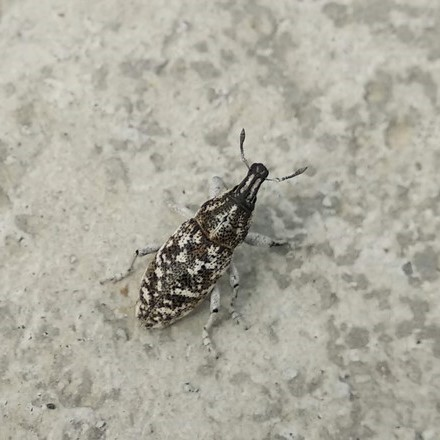
\includegraphics[width=0.49\linewidth,height=0.2\textheight]{insect_images/cyphocleonus_11} 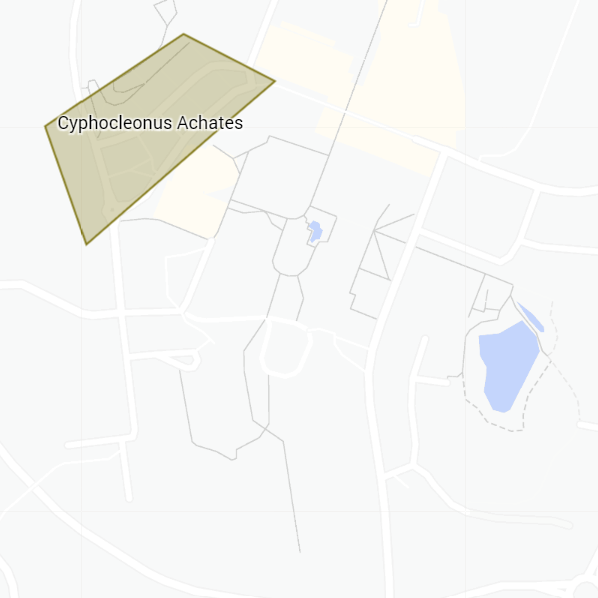
\includegraphics[width=0.49\linewidth,height=0.2\textheight]{insect_images/cyphocleonus_hotspot_11} 

}

\caption{Image of Cyphocleonus Achates. Image taken by [malreux](https://www.inaturalist.org/photos/24907280), CC BY-NC 4.0 <https://creativecommons.org/licenses/by-nc/4.0/>, via iNaturalist. Hot spot for Cyphocleonus Achates on campus.}\label{fig:unnamed-chunk-1}
\end{figure}

\hypertarget{european-mantis}{%
\section{European Mantis}\label{european-mantis}}

While this member of the Mantidae family may seem delicate, it is anything but; from the female eating the male's head after mating to the fact that it is an invasive species to North America, this insect is quite the pest. It was first introduced into North America in the 1900s as a biocontrol agent for gypsy moths but has since spread throughout the continent; this is a problem as it predates native insects, disrupting the local ecosystem.

\begin{figure}

{\centering 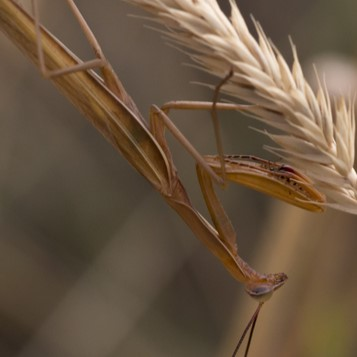
\includegraphics[width=0.49\linewidth,height=0.2\textheight]{insect_images/mantis_11} 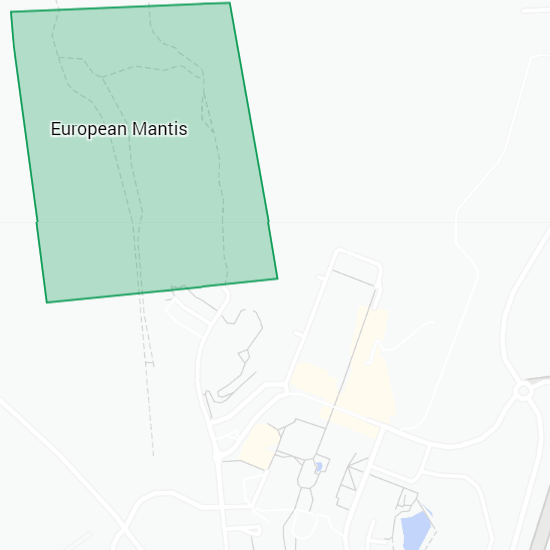
\includegraphics[width=0.49\linewidth,height=0.2\textheight]{insect_images/mantis_hotspot_11} 

}

\caption{Image of European Mantis (Mantis religiosa). Image taken by [Bob Lalonde](https://www.inaturalist.org/photos/60515212), CC BY-NC 4.0 <https://creativecommons.org/licenses/by-nc/4.0/>, via iNaturalist. Hot spot for European Mantis on campus.}\label{fig:unnamed-chunk-2}
\end{figure}

\hypertarget{asian-lady-bug}{%
\section{Asian Lady Bug}\label{asian-lady-bug}}

The Asian ladybug is a fascinating insect that has become a common sight in North America, including right here on campus. Originally introduced as a biological control for pests, such as aphids, this ladybug has since become well-established in many regions. These insects are quite different from the native ladybugs that most people are familiar with, as they can vary in coloration from orange to black and even have spots or stripes. They also have a peculiar habit of aggregating in large numbers during the fall, often seeking shelter in buildings and homes. While they may provide some benefits as predators of pests, their impact on native ladybug species and potential harm to agricultural crops is still being studied by ecologists.

\begin{figure}

{\centering 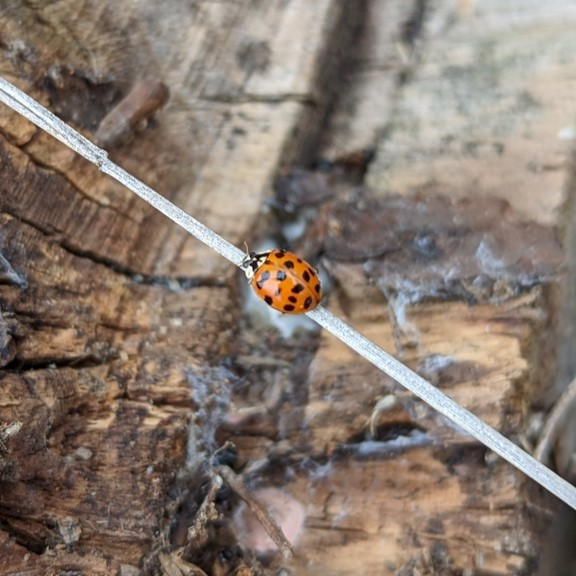
\includegraphics[width=0.49\linewidth,height=0.2\textheight]{insect_images/lady_11} 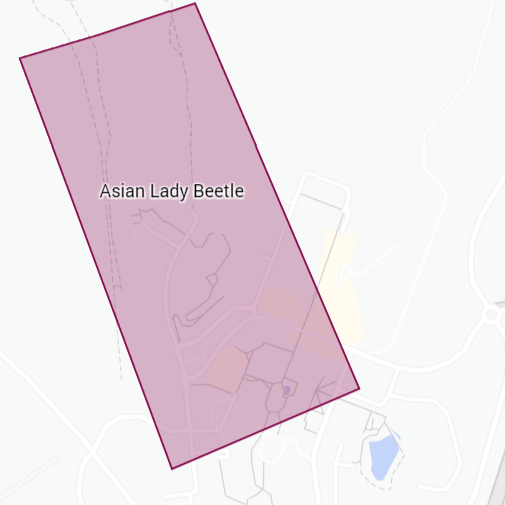
\includegraphics[width=0.49\linewidth,height=0.2\textheight]{insect_images/lady_hotspot_11} 

}

\caption{Image of Asian Lady Bug (Harmonia axyridis). Image taken by [kalvinchan](https://www.inaturalist.org/photos/230709327), CC BY-NC 4.0 <https://creativecommons.org/licenses/by/4.0/>, via iNaturalist. Hot spot for Asian Lady Bug on campus.}\label{fig:unnamed-chunk-3}
\end{figure}

\hypertarget{leopard-slug}{%
\section{Leopard Slug}\label{leopard-slug}}

Welcome to the world of the Leopard Slug, a slimy and fascinating creature that is sure to capture your attention! This impressive gastropod, also known as Limax maximus, is a true wonder of the animal kingdom. With its distinctive leopard-like spots and elongated body that can stretch up to 8 inches long, it's hard to miss this incredible slug. Found in various parts of the world, including Europe, Asia, and North America, the Leopard Slug is not your average garden pest. Instead, it's a master of disguise, using its unique coloration and shape to blend seamlessly into its surroundings. So if you're ready to learn more about this slimy superstar, keep an eye out when your walking around campus next time it rains!

\begin{figure}

{\centering 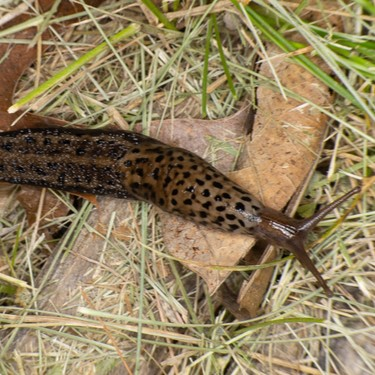
\includegraphics[width=0.49\linewidth,height=0.2\textheight]{insect_images/slug_11} 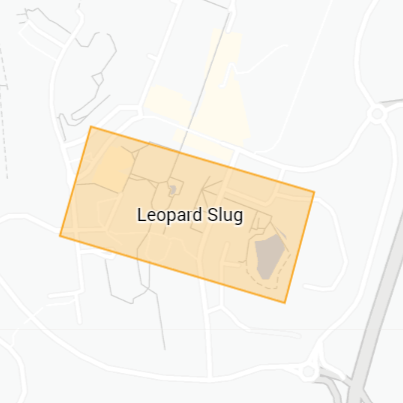
\includegraphics[width=0.49\linewidth,height=0.2\textheight]{insect_images/slug_hotspot_11} 

}

\caption{Image of Leopard Slug (Limax maximus). Image taken by [Jason Alexander](https://www.inaturalist.org/photos/80439924), CC BY-NC 4.0 <https://creativecommons.org/licenses/by-nc/4.0/>, via iNaturalist. Hot spot for Leopard Slug on campus.}\label{fig:unnamed-chunk-4}
\end{figure}

\hypertarget{california-broad-necked-beetle}{%
\section{California Broad Necked Beetle}\label{california-broad-necked-beetle}}

The California broad-necked beetle is a stunning insect that is native to the western region of North America. This beetle is around 12-15mm in length and has a unique shape that sets it apart from other beetles. Its broad, flattened neck gives it an almost distinct hourglass shape and its metallic green coloration adds to its beauty. The California broad-necked beetle can usually be found on the flowers and foliage of oak trees, primarily in the late spring and early summer months. It serves as an important part of the ecosystem by pollinating and aiding in the decomposition process. Sightings have been spread all throughout campus even up on Old Pine Trail so watch your step!

\begin{figure}

{\centering 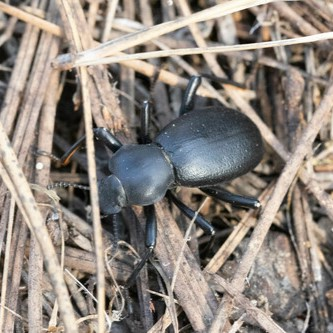
\includegraphics[width=0.49\linewidth,height=0.2\textheight]{insect_images/cali_beet_11} 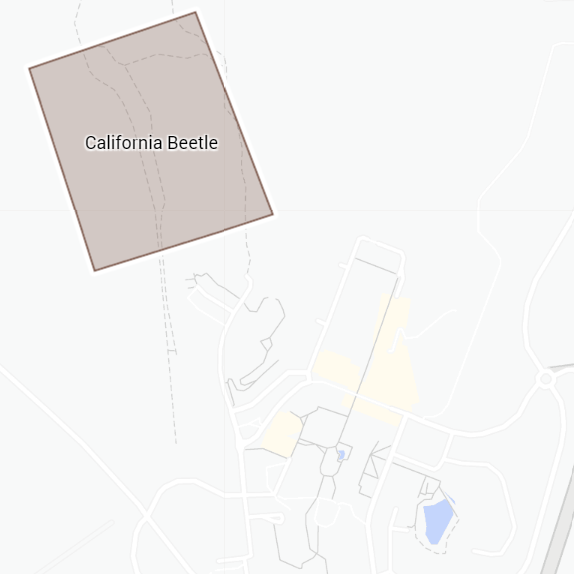
\includegraphics[width=0.49\linewidth,height=0.2\textheight]{insect_images/cali_beet_hotspot_11} 

}

\caption{Image of California broad-necked beetle (Coelocnemis dilaticollis). Image taken by [kalvinchan](https://www.inaturalist.org/photos/233670239), CC BY-NC 4.0 <https://creativecommons.org/licenses/by/4.0/>, via iNaturalist. Hot spot for California broad-necked beetle on campus.}\label{fig:unnamed-chunk-5}
\end{figure}

\hypertarget{location}{%
\section{Location}\label{location}}

\hypertarget{plantsfungi}{%
\chapter{Plants/Fungi}\label{plantsfungi}}

Campus is home to many fantastic plant species! Below we will explore just a few of our favorites.

\hypertarget{horse-chestnut}{%
\section{Horse Chestnut}\label{horse-chestnut}}

Horse chestnut is a majestic tree that can reach up to 100 feet tall. It is a native species of the Balkans and was introduced to other parts of Europe and North America in the 16th century. Horse chestnut provides food and shelter for a variety of animals, including bees, birds, squirrels, and deer. For the microbio majors out there, it can be used to extract aesculin, a glucoside that is hydrolyzed by Enterococcus making it useful for detection assays! Its large leaves and abundant flowers contribute to soil health and reduce erosion. Overall, horse chestnut is an intriguing plant with a rich cultural and ecological significance that deserves our attention and protection.

\begin{figure}

{\centering 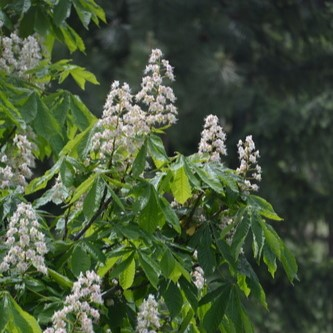
\includegraphics[width=0.49\linewidth,height=0.2\textheight]{plant_images/horse_c_11} 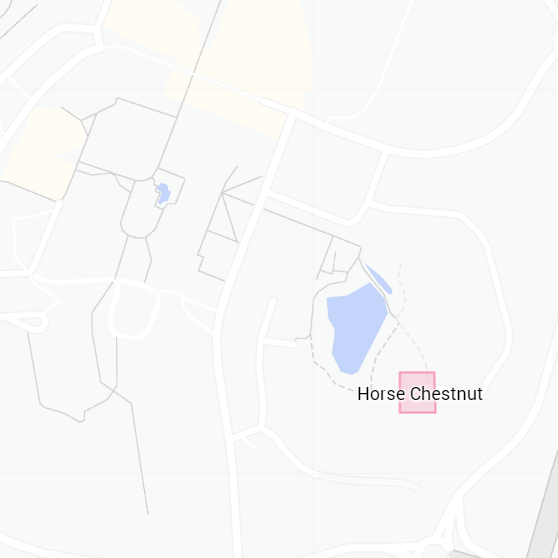
\includegraphics[width=0.49\linewidth,height=0.2\textheight]{plant_images/horse_c_hotspot_11} 

}

\caption{Image of Horse Chestnut (Aesculus hippocastanum). Image taken by [lesfreck](https://www.inaturalist.org/photos/201399267), CC BY-NC 4.0 <https://creativecommons.org/licenses/by-nc/4.0/>, via iNaturalist. Hot spot for Horse-Chestnut on campus.}\label{fig:unnamed-chunk-6}
\end{figure}

\hypertarget{bonnets}{%
\section{Bonnets}\label{bonnets}}

Bonnets are marvels of nature! These beautiful, bulbous fungi boast delicate petals that punctuate their round, globe-like shape. They're a vital part of our planet's intricate ecological web, providing nourishment and shelter for a wide array of creatures.Some species of bonnets are also known to have medicinal properties, making them valuable not just for their aesthetic appeal, but for their contributions to the health of our planet; their ediblity isn't known for a lot of species so maybe don't use them for your ravioli. Take a moment to appreciate the intricate beauty of bonnets as you walk along the EME pond or Old Pine Trail, and you'll see just how wondrous and important these plants truly are.

\begin{figure}

{\centering 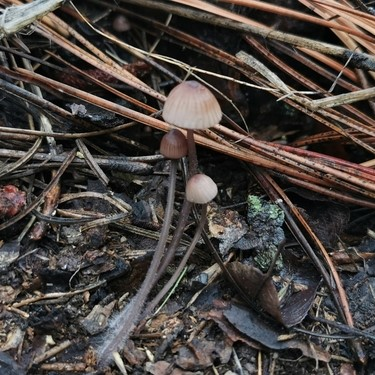
\includegraphics[width=0.49\linewidth,height=0.2\textheight]{plant_images/bonnets_11} 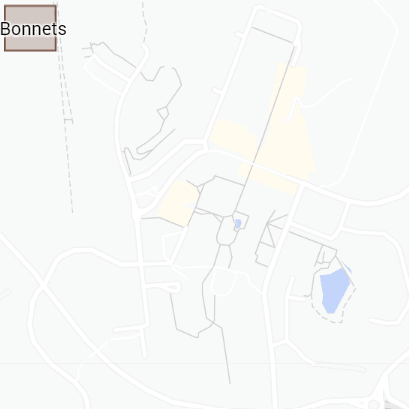
\includegraphics[width=0.49\linewidth,height=0.2\textheight]{plant_images/bonnets_hotspot_11} 

}

\caption{Image of Bonnets (Genus Mycena). Image taken by [kalvinchan](https://www.inaturalist.org/photos/170911702), CC BY-NC 4.0 <https://creativecommons.org/licenses/by-nc/4.0/>, via iNaturalist. Hot spot for bonnets on campus.}\label{fig:unnamed-chunk-7}
\end{figure}

\hypertarget{silvery-cinquefoil}{%
\section{Silvery Cinquefoil}\label{silvery-cinquefoil}}

Silvery cinquefoil is a striking silver-leaved plant that looks like it's out of a fairytale. This subalpine plant has delicate five-petaled yellow flowers that bloom in dense clusters on long stems that reach about 20 cm tall. The angled, five-toothed leaves are covered with fine silver hairs on the bottom, creating a unique shimmering effect that catches the eye. Despite its small size and delicate appearance, silvery cinquefoil is a tough survivor that thrives in harsh, rocky environments. It's a plant that embodies the magic and resilience of nature; despite its alluring appearance, it is considered a pest as it is an introduced species from Eurasia.

\begin{figure}

{\centering 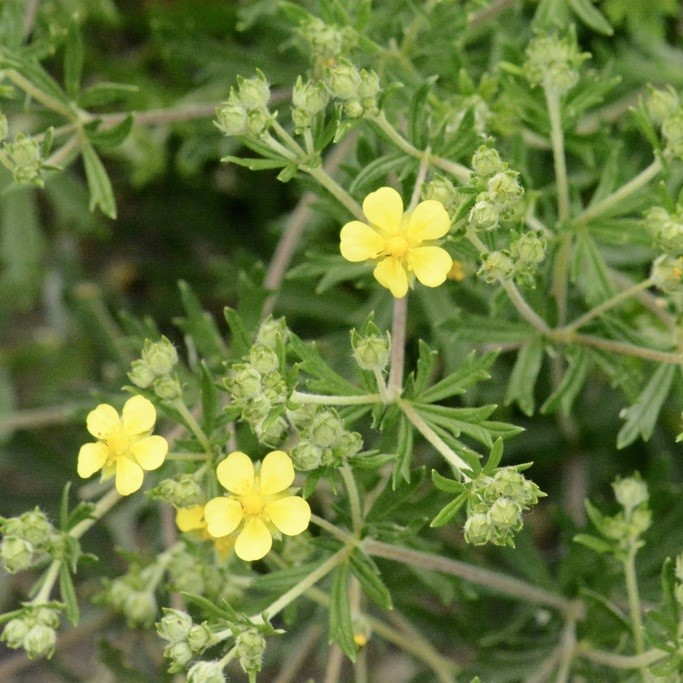
\includegraphics[width=0.49\linewidth,height=0.2\textheight]{plant_images/silvery_cinq_11} 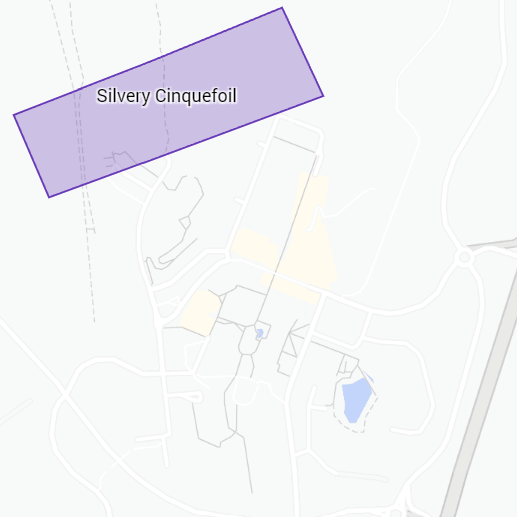
\includegraphics[width=0.49\linewidth,height=0.2\textheight]{plant_images/silveryconquefoil_hotspot_11} 

}

\caption{Image of Silvery Cinquefoil (Potentilla argentea). Image taken by [lesfreck](https://www.inaturalist.org/photos/198692554), CC BY-NC 4.0 <https://creativecommons.org/licenses/by-nc/4.0/>, via iNaturalist. Hot spot for Silvery Cinquefoil on campus.}\label{fig:unnamed-chunk-8}
\end{figure}

\hypertarget{bittersweet-nightshade}{%
\section{Bittersweet Nightshade}\label{bittersweet-nightshade}}

Bittersweet nightshade is a fascinating perennial plant that belongs to the nightshade family. This plant boasts small, star-shaped purple or white flowers that give way to shiny, red berries. Beware, though, as their bright and juicy berries can be tempting, their hollow stem and leaves contain a bitter toxin that can cause nausea, vomiting, and even hallucinations. Native to Asia and Europe, bittersweet nightshade has a long history of traditional medicinal use, but it is also a standout in the world of ecology. Due to its aggressive nature and ability to adapt to a wide range of habitats, bittersweet nightshade is classified as an invasive species in many regions including the Thompson-Okanagan. So while its beauty and intrigue may be captivating, it's important to remember that bittersweet nightshade is a complex and potentially dangerous plant that serves as a reminder of the delicate balance of our natural world. Be sure to be on the lookout next time you take a study break around the pound behind EME!

\begin{figure}

{\centering 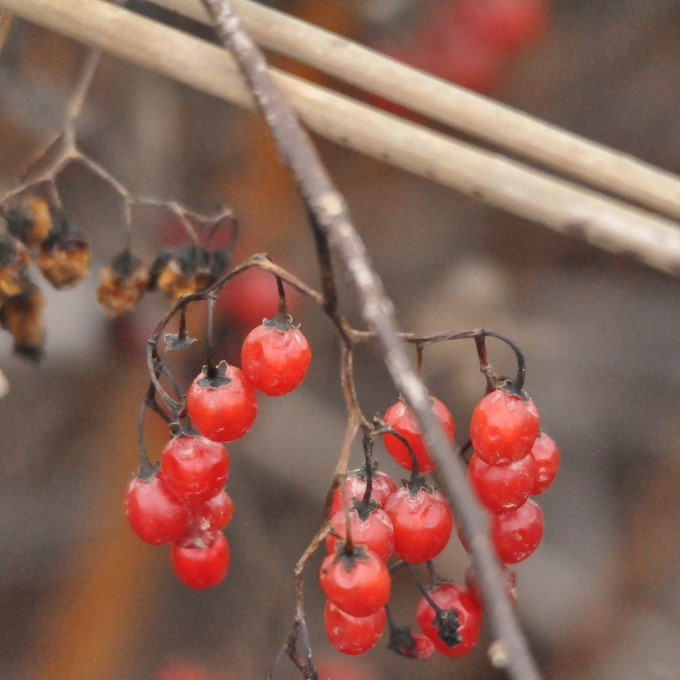
\includegraphics[width=0.31\linewidth,height=0.2\textheight]{plant_images/bitter_night_red_11} 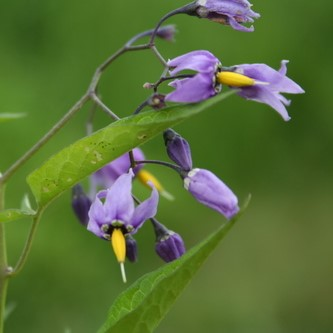
\includegraphics[width=0.31\linewidth,height=0.2\textheight]{plant_images/bitter_night_purp_11} 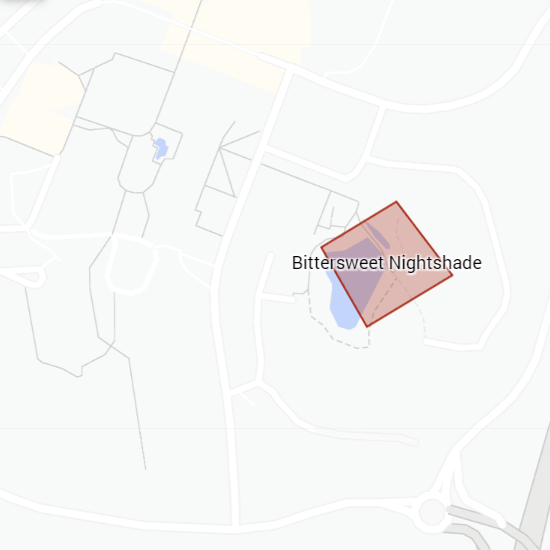
\includegraphics[width=0.31\linewidth,height=0.2\textheight]{plant_images/bitter_night_hotspot_11} 

}

\caption{Images of Bittersweet Nightshade (Solanum dulcamara). Left most image taken by [lesfreck](https://www.inaturalist.org/photos/61694401), CC BY-NC 4.0 <https://creativecommons.org/licenses/by-nc/4.0/>, via iNaturalist. Middle image taken by [Alexander Baransky](https://www.inaturalist.org/photos/70860715), CC BY-NC 4.0, via iNaturalist. Hot spot for Bittersweet Nightshade on campus.}\label{fig:unnamed-chunk-9}
\end{figure}

\hypertarget{wolf-lichen}{%
\section{Wolf Lichen}\label{wolf-lichen}}

Wolf lichen is yellow-green in colour, shrubby and highly branched. It most often grows on the bark of living and dead conifers. The pigment that gives wolf lichen its yellow colour (vulpinic acid) is slightly toxic to mammals. The toxic pigment was used historically to poison wolves, which is the inspiration for the name wolf lichen.

\begin{figure}

{\centering 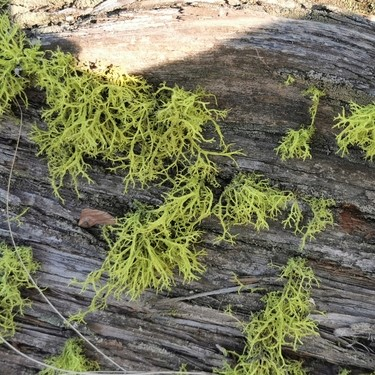
\includegraphics[width=0.49\linewidth,height=0.2\textheight]{plant_images/wolf_inat_11} 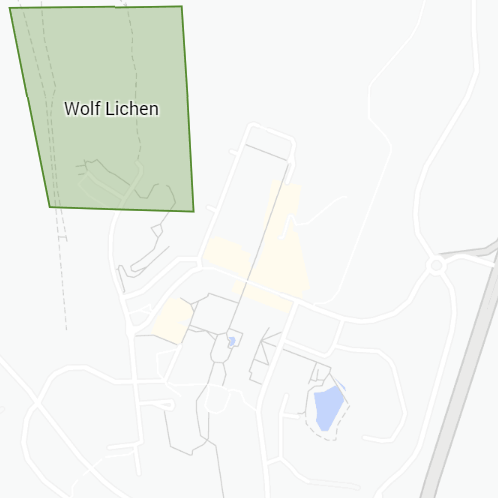
\includegraphics[width=0.49\linewidth,height=0.2\textheight]{plant_images/wolflichen_hotspot_11} 

}

\caption{Image of Wolf Lichen (Letharia vulpina). Image taken by [kalvinchan](https://www.inaturalist.org/photos/179070916), CC BY-NC 4.0 <https://creativecommons.org/licenses/by-nc/4.0/>, via iNaturalist. Hot spot for Wolf Lichen on campus.}\label{fig:unnamed-chunk-10}
\end{figure}

\hypertarget{location-1}{%
\section{Location}\label{location-1}}

  \bibliography{book.bib,packages.bib}

\end{document}
